\section{Signal and Background Classification}

\subsection{Sideband-labelled samples}

The signal/background study uses mass windows to create approximate labels. Candidates in a narrow window around the B mass are labelled as signal-like, while candidates in lower and upper mass sidebands are labelled as background-like. The sideband method is common in HEP because sideband regions provide a data-driven representation of combinatorial background.

The label definition used in the notebook is
\begin{align}
  \mathrm{signal:} \qquad & 5270 < m_B < 5290~\mevcc, \\
  \mathrm{background:} \qquad & 5200 < m_B < 5250~\mevcc \quad \mathrm{or} \quad
  5310 < m_B < 5350~\mevcc .
\end{align}
These labels are proxy labels. The signal window can still contain background, and the sidebands may not perfectly represent the background under the signal peak. Nevertheless, the construction is useful for demonstrating a realistic machine-learning workflow without relying on simulation truth information.

\subsection{Random Forest classifier}

A Random Forest classifier~\cite{sklearn} is trained using reconstruction-quality and PID variables. The B-candidate mass is deliberately excluded from the feature list, because the mass defines the labels. Including it would make the classifier learn the sideband construction rather than physically meaningful differences in candidate quality or PID response.

The classifier uses the following feature set:
\begin{equation}
  \left\{
  \chi^2_{\mathrm{vertex}}(B),\,
  d_{\mathrm{flight}}(B),\,
  P_K(H_1), P_K(H_2), P_K(H_3),\,
  P_{\pi}(H_1), P_{\pi}(H_2), P_{\pi}(H_3)
  \right\}.
\end{equation}
The label construction yields $528$ signal-like and $227$ background-like
candidates, and the model is evaluated on a held-out third of that sample
($227$ candidates). The receiver operating characteristic (ROC) curve in
Fig.~\ref{fig:roc} shows the trade-off between signal efficiency and background
misclassification rate. The diagonal line corresponds to a classifier with no
discriminating power.

\begin{figure}[H]
  \centering
  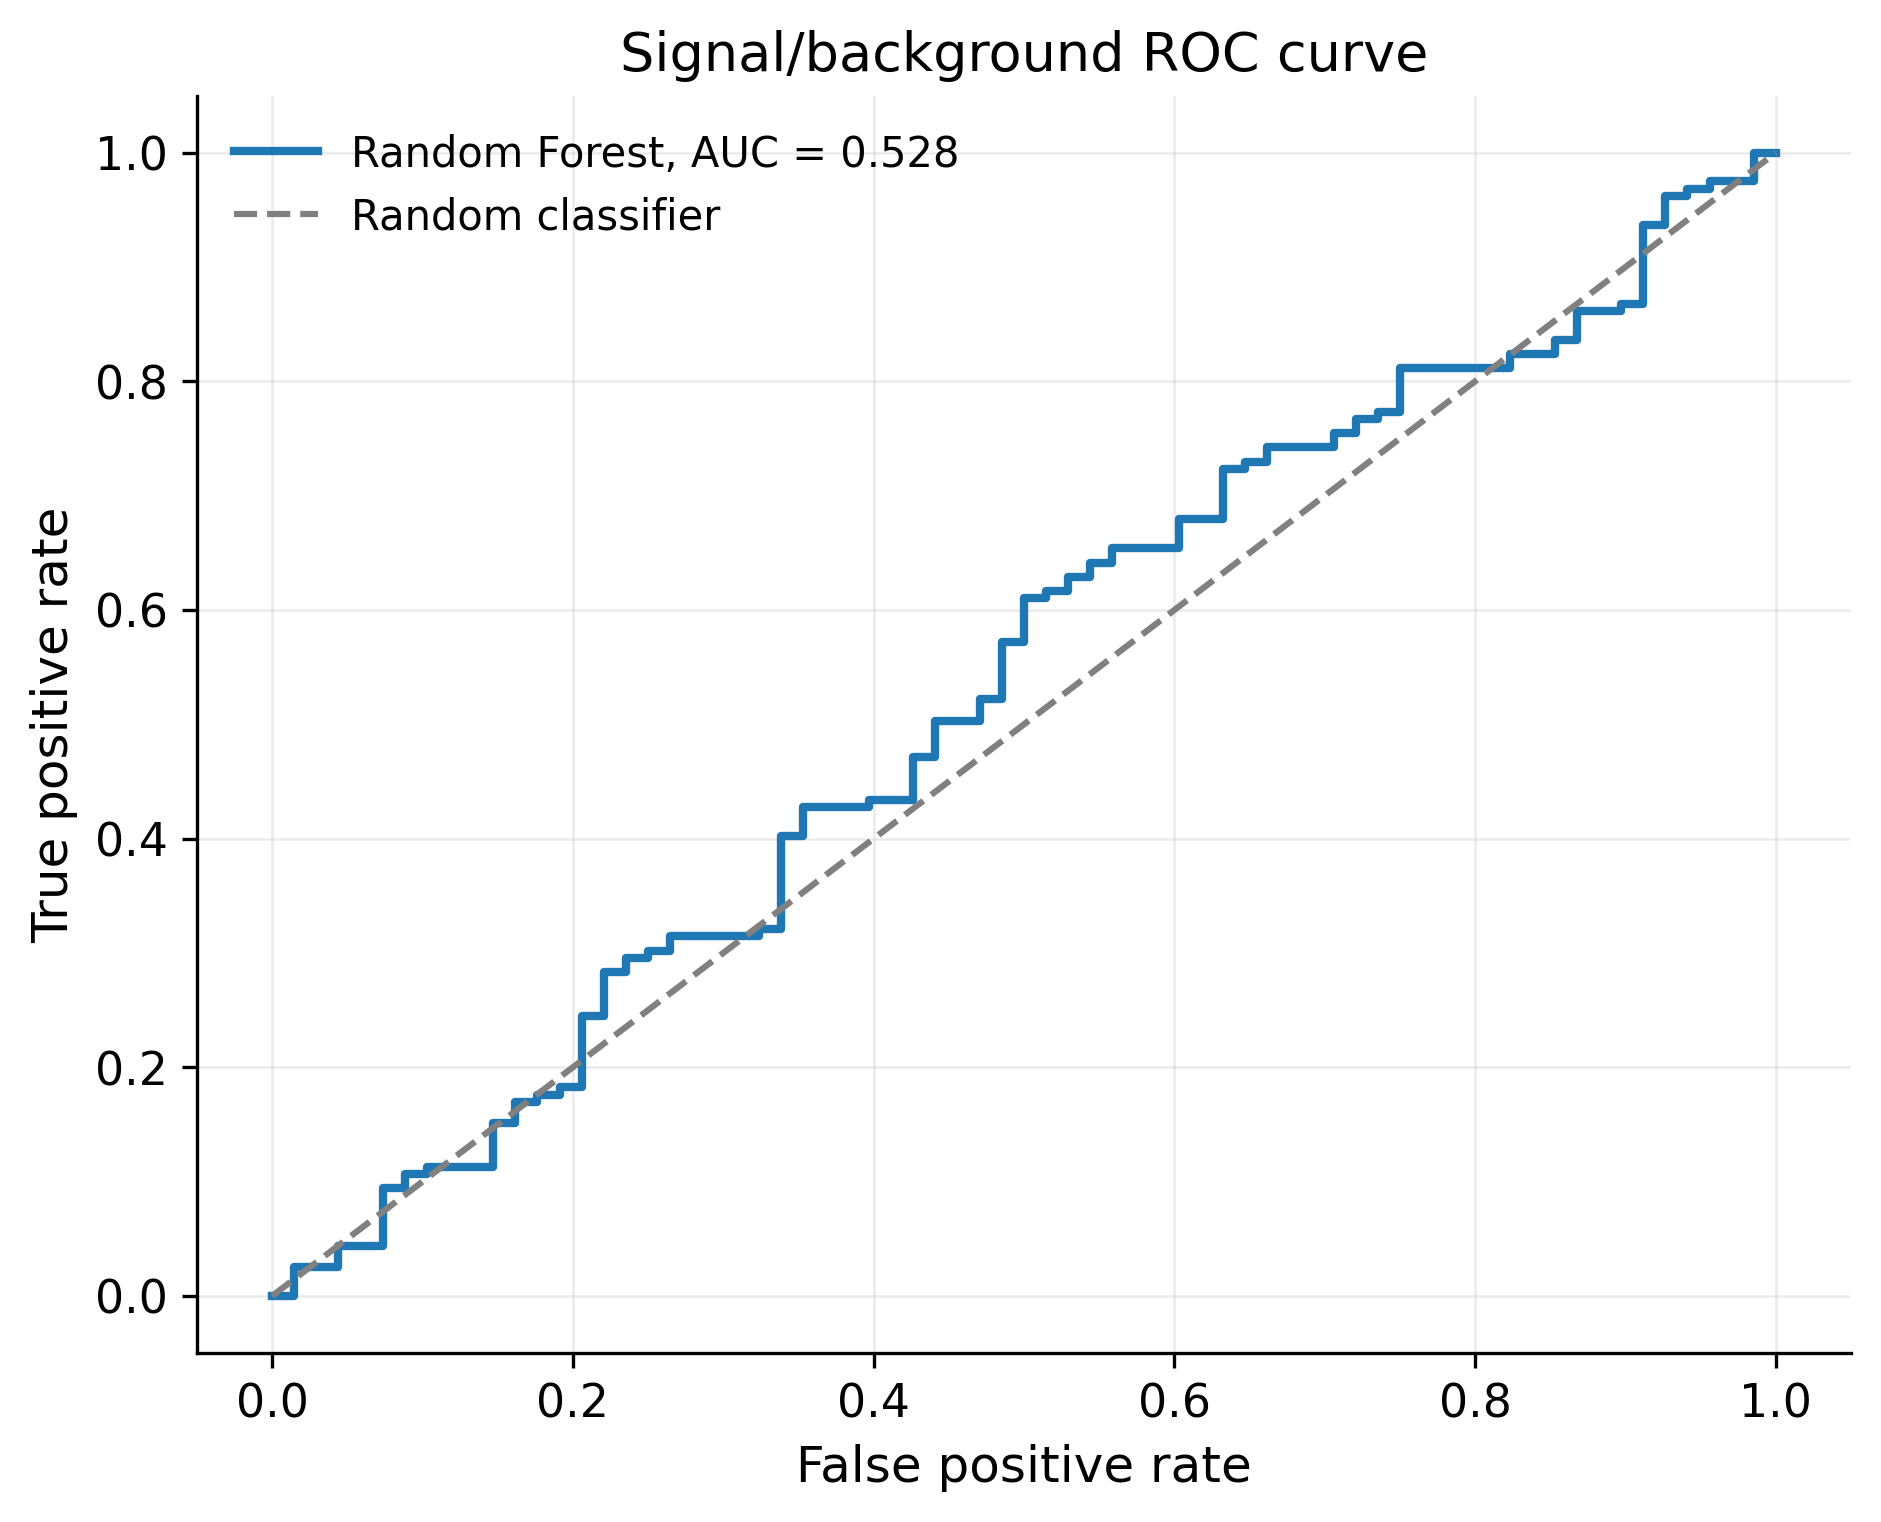
\includegraphics[width=0.75\textwidth]{roc_signal_background.png}
  \caption{ROC curve for the sideband-labelled Random Forest signal/background classifier.}
  \label{fig:roc}
\end{figure}

The measured area under the curve is $\mathrm{AUC}=0.528$. This is compatible
with no separation at all, and it should be read as a negative result rather than
as a performance figure. Two reasons explain it, and both are properties of the
analysis rather than of the algorithm. First, the baseline selection of
Sec.~\ref{sec:selection_effect} is already tight enough that the surviving sample
is dominated by signal; the classifier is asked to separate a background
population that has largely been removed. Second, the features available in the
ntuple are the same variables the selection already cuts on, so little
independent information is left. Training before the tight preselection, on a
looser sample and with additional kinematic variables, is the way to make this
study informative; it is listed as a planned extension.

Figure~\ref{fig:feature_importance} shows the feature-importance ranking from the Random Forest model. Given the AUC above, this ranking describes which variables the model used, not which variables carry physical discrimination. Such rankings depend on feature correlations, sample composition, and the chosen model architecture, and should not be read as physics observables.

\begin{figure}[H]
  \centering
  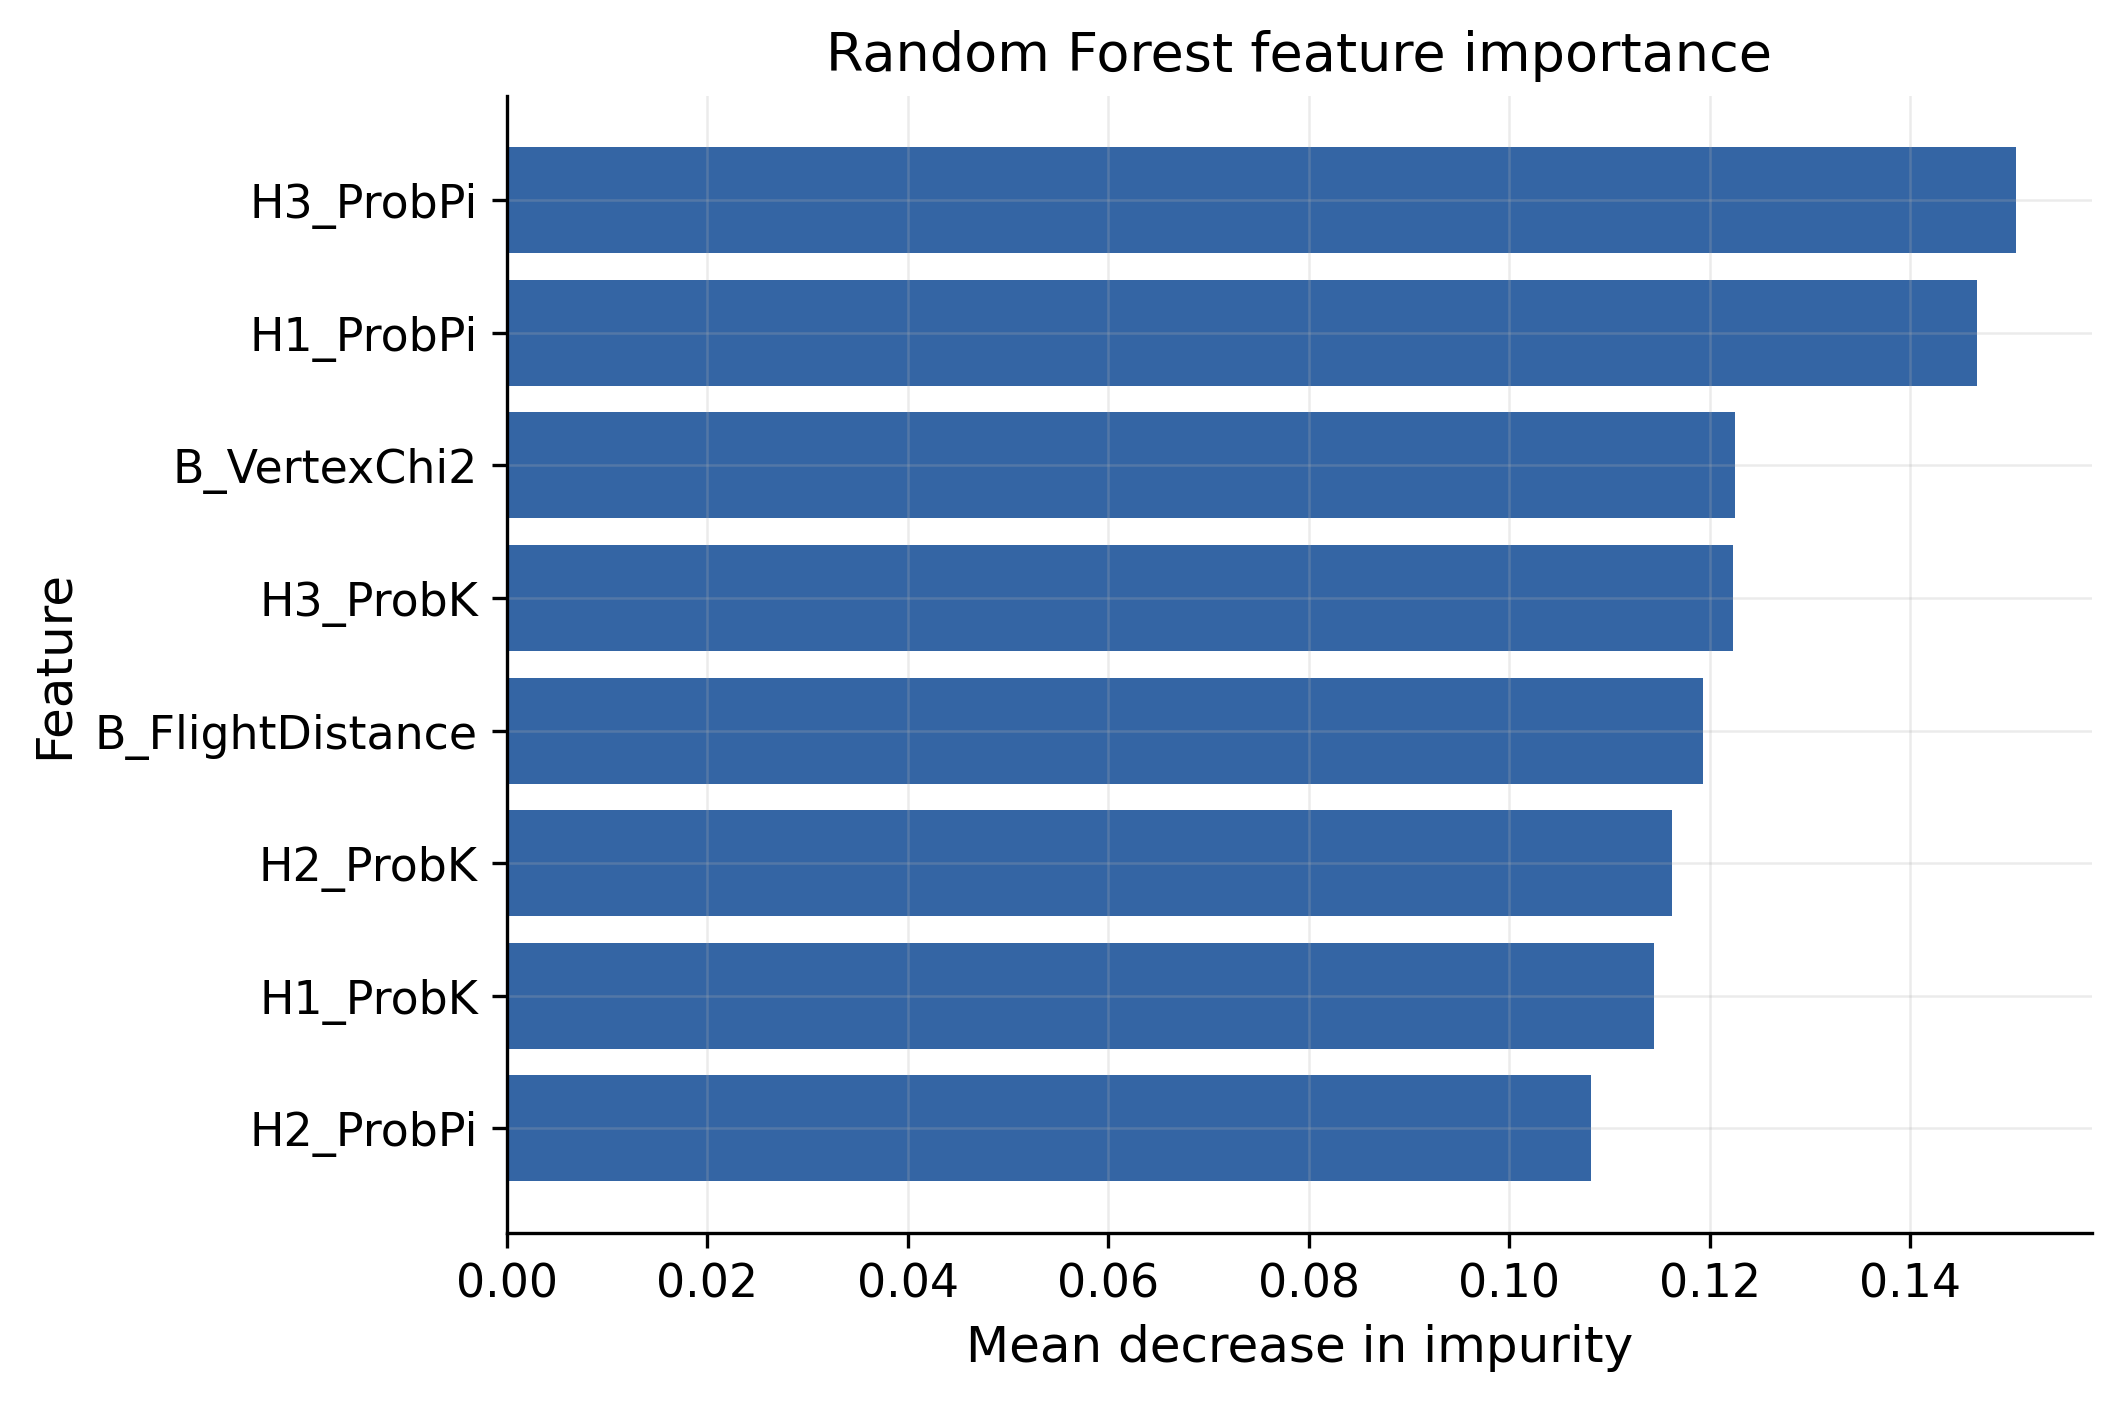
\includegraphics[width=0.82\textwidth]{feature_importance_signal_background.png}
  \caption{Random Forest feature importance for the signal/background classification task.}
  \label{fig:feature_importance}
\end{figure}

This part of the project demonstrates the integration of standard HEP sideband logic with modern machine-learning tools, and it also demonstrates when such a tool has nothing to add. The classifier is not used anywhere in the mass-fit, asymmetry or Dalitz results that follow; those rely on the transparent baseline selection alone. Making the classification study useful would require training before the preselection, cross-validation, gradient-boosted decision trees, systematic studies of the sideband definition, and comparisons with simulation.
